\chapter{Proposed Solution}
\label{chap:solution}

In this chapter, a proposal is presented that attempts to address the security issues of OBD-II. This system employs all the security related solutions of chapter \ref{chap:preliminaries} in it's design. More specifically the concept of RBAC is applied to the OBD-II interface, in an effort to address it's wide open nature. First, a general description of the ideal OBD-II system is presented (i.e. a OBD-II system that doesn't suffer from all the problems mentioned in \ref{chap:problem_statement}). Next, the design of the proposed solution is discussed.

\section{Ideal OBD-II System}
\label{sec:sol_RBAC}

They key research question here is: can a solution be developed that would protect an in-vehicle network from unauthorised access via the OBD-II port. The concept of 'unauthorised access' is key, since the goal is not to deny access altogether. Only authorised personnel (e.g. repairmen) should be allowed high levels of access. Meaning that only they should be allowed to start diagnostic sessions, recalibrate ECU's, etc. The only way of differentiating between what is allowed and what isn't is by looking at the messages that are sent, specifically their ID. Some messages, like a message asking for the status of a certain ECU could be considered harmless. The message that is used to initiate a diagnostics session however is not that innocent, since it is shown in \cite{MillerC} that this could be used to disengage the brakes, kill the engine, etc. It follows that any solution to this problem should involve a series of authorisation levels and that each of these is associated with a number of permitted message ID's. The concept of role-based access control (see \ref{sec:RBAC}) is clearly applicable here. \\ \\ The next question to answer is where this system of access control is enforced. The assertion made in section \ref{sec:current_state}, stating that the main problem of OBD-II is the indiscriminate nature at which the gateway forwards messages coming from the interface, hints at the ideal solution. Because of it's strategic position and privileged role in forwarding messages, the gateway is the ideal location to enforce a RBAC system for OBD-II. \\ \\ The final question is how to enforce RBAC in practice. In a common enterprise RBAC system the worker authenticates to the system via some type of authentication key. this key can be literal: physical key, key-card, software key, etc. However, in some instances this key is represented by some type of secret knowledge (like a password or PIN-code) or even some identifying characteristic of the individual (fingerprint scan, retinal scan, etc). The  worker authenticates to the system by proving he/she is in possession of the appropriate key. Translating this concept to our situation the user (e.g. car owner, repairman, policeman, etc) authenticates him-or-herself by proving to the system (the gateway of the vehicle) that he or she is in possession of the appropriate key. The system will verify this key before granting the permissions that correspond to the appropriate role. It should come as no surprise that an authentication scheme based on software keys is appropriate here.


Every authorisation level constitutes a role, and what messages are allowed for each level constitute the permissions of this role. More specifically this system should be considered an instance of mandatory access control, since the users are not allowed any control over what permissions they are granted. Now that a system of access control is introduced, we need to look at how this system can be implemented to protect the OBD-II port.

\section{OBD-II Access Control}
\label{sec:obd2_access_control}

It's time to present our solution. Our proposal constitutes a RBAC system for the OBD-II interface, that employs asymmetric key pairs to authenticate users. This system is illustrated in \ref{fig:solution}. The choice was made to make use of cryptographic keys to implement access control as well as associating a different security policy (and by extension different keys) for every car model. From section \ref{sec:PKC} it follows that there are two cryptographic key technologies that can be considered: symmetric and asymmetric. Symmetric cryptography has the advantage of shorter key lengths, however this would entail that if the keys of one vehicle were extracted (e.g. by extracting and analysing the gateway) and distributed, all vehicles of the same model would be compromised. That is why the decision was made to use asymmetric keys. \\ \\ The gateway stores a series of public keys, each associated with a specific role. A user wishing to authenticate would have to prove ownership of the appropriate private key. This key ownership configuration could be flipped (i.e. gateway stores private key and user owns public key). However, this configuration has the same major design flaw that symmetric encryption had, namely possible extraction of the private key from the vehicle. The decision to use asymmetric keys moves the responsibility of safely storing the private key to the users. Intuitively this might seem worse, since now the private keys are already in the hands of individuals. Individuals that might have ulterior motives concerning their level of access. This flaw was countered by introducing a central server that safely stores the private keys, together with an internet connected device called a tester that physically connects to the OBD-II port. Users with privileged roles will first authenticate to the central server via the tester, using some other authentication method (e.g. login and password). This dedicated device will then initiate an authentication procedure with the gateway, proving ownership of the appropriate private key. This authentication procedure is discussed in more detail next.

\begin{figure}[h]
	\label{fig:solution}
	\centering
	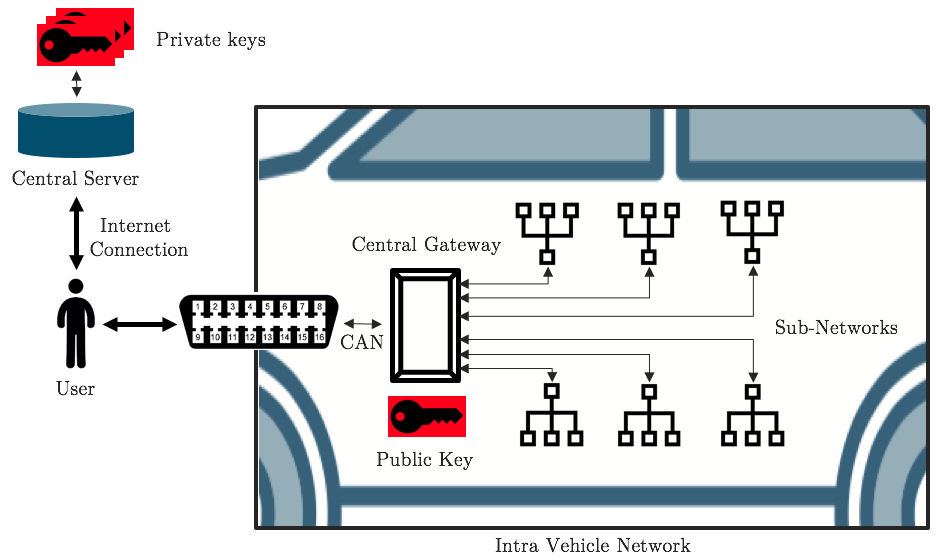
\includegraphics[width=\textwidth]{solution.png}
	\caption{OBD-II access control architecture.}
\end{figure}


\subsection{Authentication Procedure}
\label{subsec:authentication_procedure}

The goal of the authentication procedure to prove to the gateway possession of the appropriate private key. The choice was made to initiate an authenticated session between tester and gateway by calculating a shared secret key. This calculation would incorporate the pre-shared asymmetric keys, thereby combining authentication and secret key establishment into a single procedure. This procedure is based on the ECDHE\_ECDSA algorithm introduced in section \ref{subsubsec:ecdh_ecdsa}, more specifically figure \ref{fig:ECDH2}. A couple of changes were applied to this algorithm to more closely adhere to our situation:
\begin{enumerate}
	\item \textbf{Gateway Key Pair:} A precondition for the ECDHE\_ECDSA algorithm is that both parties have an ECC key pair already established. For the tester this condition is already met. Even better, the corresponding public key is already given to the gateway. For the gateway however this is not the case. Since ECDH requires two key pairs, a new key pair will have to computed every time the procedure is run.
	
	\item \textbf{Perfect Forward Secrecy:} We can get rid of the ephemeral keys. This is because perfect forward secrecy (or secrecy in general) is not a goal in our situation. the goal is to protect against unauthorised access, not to protect past sessions from leaking. 
	
	\item \textbf{Mutual Authentication:} The first authentication step can be omitted (i.e signing by the gateway, and verification by the tester). Because of the absence of a gateway key pair, it is impossible for the gateway to authenticate itself to the tester. Moreover, this is not even a requirement of our authentication procedure.
\end{enumerate}
Applying all of these modifications the procedure from figure \ref{fig:authentication_procedure} is obtained. Before the procedure is initiated the central server is in possession of the OBD-II private key $Pr_{obd}$, while the gateway has the appropriate public key $Pb_{obd}$ stored in memory. The user of the tester initiates the procedure by connecting to the OBD-II DLC, after which the tester sends an initialization message to the gateway. This initialization message also specifies the role that the user of the tester wishes to authenticate as. The gateway responds to this by creating a new ECC key pair: KGen($Pb_g$,$Pr_g$), and sending the newly created public key $Pb_g$ to the tester. The tester then forwards this secret key to the central server, which in turn signs this public key using the OBD-II private key: Sig($Pb_g$,$Pr_{obd}$), before sending the signature back to the tester. The tester then forwards this signature (only the signature) back to the gateway. After the gateway has verified the signature using the OBD-II private key: Ver(Sig,$Pb_{obd}$), both parties calculate the shared secret using ECDH. The gateway does so on his own: $K$=ECDH($Pr_g$,$Pb_{obd}$). The tester however does not have all the ingredients to do so, since the OBD private key is stored on the central server. That is why it is generated on the server, and securely sent to the tester. This newly created secret can then be used to authenticate every OBD-II message that is sent in the upcoming session. This procedure is discussed next.
 
\begin{figure}[h]
	\centering
	\fbox{
		\procedure{OBD-II Authentication Procedure}{%
			\textbf{Central Server} \<\< \textbf{Tester}  \<\< \textbf{Gateway} \\
			\text{$Pr_{obd}$} \<\<\<\< \text{$Pb_{obd}$} \\
			\<\< \< \sendmessageright{length=1.5cm,top=\text{init}} \<\\
			\<\<\<\< \text{KGen($Pb_g$,$Pr_g$)} \\
			\<\sendmessageleft{length=1.5cm,top=\text{$Pb_g$}} \<\< \sendmessageleft{length=1.5cm,top=\text{$Pb_g$}} \<\\
			\text{$S$=Sig($Pb_g$,$Pr_{obd}$)} \<\<\<\< \\
			\< \sendmessageright{length=1.5cm,top=\text{$S$}} \<\< \sendmessageright{length=1.5cm,top=\text{$S$}} \<\\
			\<\<\<\< \text{Ver($S$,$Pb_{obd}$)} \\
			\text{$K$=ECDH($Pr_{obd}$,$Pb_g$)} \< \sendmessageright{length=1.5cm,top=\text{$K$}} \<\<\< \text{$K$=ECDH($Pr_g$,$Pb_{obd}$)} \\
		}
	}
	\caption{OBD-II Authentication Procedure}
	\label{fig:authentication_procedure}
\end{figure}

\subsection{Message Authentication}
\label{subsec:message_authentication}

The authentication procedure from section \ref{sec:authentication_procedure} authenticates the tester to the gateway, thereby also establishing a shared secret. The next step is to design a procedure that uses this shared secret to facilitate an authenticated communications session. The solution proposed by the researchers of this paper is simple and illustrated in figure \ref{fig:message_authentication}. The OBD-II message sent by the tester ($M$) is followed up by a message containing a MAC: MAC($M$,$K$) (see section \ref{sec:MAC}). This MAC is calculated by inputting the data of the first CAN frame as well as the recently established secret key $K$. Before the gateway forwards the message to the appropriate sub-network, it first performs two distinct security checks: 
\begin{itemize}
	\item \textbf{Permissions Check} CheckP($M$): This is where the role based access control system proposed in section \ref{sec:sol_RBAC} is actually enforced. The gateway knows what role the tester authenticated as, so the first condition that is checked is whether this role has permission to send the message $M$. It will do this this by looking up the ID of the message in the permissions table (see section \ref{sec:permissions_table}). If the message ID is not present, the message will be denied and the tester (and by extension the user) is notified.
	
	\item \textbf{MAC Verification} Ver(MAC,$K$): After the message $M$ passes the permissions check, the gateway will check whether the received MAC is correct. This way ensuring that the sender of this message is authorized. Again, if this test fails the message will be denied and the tester is notified
\end{itemize}
If both these checks succeed, the OBD-II message $M$ is forwarded to the appropriate sub-network and the tester receives an acknowledgement (ACK). 

\begin{figure}[h]
	\centering
	\fbox{
		\procedure{Message Authentication}{%
			\textbf{Tester}  \<\< \textbf{Gateway} \<\< \textbf{Network}\\
			\text{$K$}  \<\< \text{$K$} \<\< \\
			\< \sendmessageright{length=3cm, top=\text{OBD-II message $M$}} \<\<\<\\
			\<\< \text{CheckP($M$)} \<\< \\
			\< \sendmessageright{length=3cm, top=\text{MAC($M$,$K$)}} \<\<\<\\
			\<\< \text{Ver(MAC,$K$)} \<\< \\
			\<\<\< \sendmessageright{length=3cm, top=\text{$M$}} \< \\
			\< \sendmessageleft{length=3cm, top=\text{ACK}} \<\<\< \\
		}
	}
	\caption{OBD-II Message Authentication}
	\label{fig:message_authentication}
\end{figure}

\subsection{Permissions Table} 
\label{subsec:sol_permissions_table}
The permissions table is stored on the gateway, and is used to determine which OBD-II messages are allowed for each role. Before looking at the design of the OBD-II permissions table, we need to concretely define the roles themselves. It is worth noting that the selection made here is purely for demonstrative purposes. Significant additional research would have to be conducted to determine what roles are necessary for this system to adhere to the current automotive landscape (TODO ref).

\begin{itemize}
	\item \textbf{Admin:} This role is not related to the intra vehicle network, but rather the OBD-II access control system itself. It is essential that the software that enforces RBAC on the gateway can be updated and configured (e.g. replacing public keys when the corresponding private key was compromised). Any user authenticating themselves as an admin will have the ability to send specific control messages that are designed to modify the existing RBAC software on the gateway.
	
	\item \textbf{OEM:} The original equipment manufacturer (OEM) refers to the company that designed and produced the various ECU's that are found inside the vehicle. By extension, the manufacturer of the vehicle itself is considered an OEM in this case. Workers authenticating themselves as an OEM need considerable control over the intra vehicle network to correctly test, configure and update ECU's. This is why this role will generally be granted a high level of clearance.
	
	\item \textbf{Repairman:} Probably the most obvious candidate for a role since OBD-II was designed first-and-foremost to diagnose and fix vehicle malfunctions. And this is exactly what repairmen are employed to do.
	
	\item \textbf{Policeman:} In section \ref{subsec:informal_model} we discussed the possibility of car owners illegally tampering with their own vehicles (e.g. reducing odometer values before selling). It is up to law enforcement to prohibit this kind of behaviour, and the most efficient way of doing so is by interfacing with the OBD-II interface. This is why policemen should be granted their own role, granting them easy access to ECU's that are frequently the subject of tampering.
	
	\item \textbf{Owner:} This role corresponds to the lowest level of clearance. The owner of the vehicle is only trusted with harmless OBD-II messages, allowing adventurous vehicle owners to safely interact with their vehicle's intra vehicle network.
\end{itemize}
The general architecture of RBAC permissions tables is as follows: every entry in the table is associated with a permission, or in this context, the ID of a specific CAN message. Each entry will have series of fields (equal to the amount of roles that are defined), and each field signals whether the corresponding permission is granted to the role of that particular field. Table \ref{table:2} shows the design of the table, with one example field.

\begin{table}[]
	\begin{tabular}{|c|c|c|c|c|c|}
		\hline
		\rowcolor[HTML]{9B9B9B} ID & Admin & OEM & Repairman & Policeman & Owner \\ \hline
		\cellcolor[HTML]{9B9B9B} IDH: 07, IDL: E0 & Yes & Yes & Yes & No & No \\ \hline
		\cellcolor[HTML]{9B9B9B} \vdots & \vdots & \vdots & \vdots & \vdots & \vdots
	\end{tabular}
	\caption{OBD-II permissions table example.}
	\label{table:2}
\end{table}

